This chapter presents a systematic review of the main theoretical
aspects involved in the construction, estimation and implementation of a
generalized linear mixed model (GLMM). We start in \autoref{cap:joint}
with the model construction framework, concluding with the so-called
joint likelihood function. \autoref{cap:laplace} address the
marginalization of that joint likelihood, performed here in terms of a
Laplace approximation technique. \autoref{cap:opt} discusses available
alternatives for the parameters optimization of the marginal likelihood
obtained through that marginalization. \autoref{cap:ad} talks about
automatic differentiation (AD), the most efficent manner of computing
derivatives, and a key point for us. Last but not least, in
\autoref{cap:tmb} we present the computational tool used to peform all
the discussed procedure, the TMB: Template Model Builder. A very
exciting \texttt{R} \cite{R18} package developed by~\citeonline{TMB}.

\section{CONSTRUCTION: JOINT LIKELIHOOD FUNCTION}
\label{cap:joint}

A GLMM models an \(n\)-vector of exponential family random variables,
\(\mathbf{Y}\), in terms of its conditional expected value, \(\bm{\mu}
\equiv \mathbb{E}(\mathbf{Y} \mid \mathbf{X}, \mathbf{u})\), via a
linear combination called of linear predictor and generally expressed by
\begin{equation}
  g(\bm{\mu}) = \mathbf{X} \bm{\beta} + \mathbf{Zu}, \quad
  \mathbf{u} \sim \mathcal{N}(\mathbf{0}, \bm{\Sigma}).
  \label{eq:gmu}
\end{equation}
In other words, a GLMM is a generalized linear model (GLM) in which the
linear predictor depends on some Gaussian latent effects,
\(\mathbf{u}\), times a latent effects model matrix \(\mathbf{Z}\).
Since we do not observe the latent component, an exemplification of the
idea embedded in matrix \(\mathbf{Z}\) is welcome. Suppose, e.g. three
individuals (or clusters) and that each one has two measures. This
configures a repeated measures context, the most common latent structure
in family studies.. Also, it is reasonable to admit that each individual
has its particular latent effect value. Consequently,
\[
  \mathbf{Zu} = \begin{bmatrix}
                 1 & 0 & 0\\1 & 0 & 0\\
                 0 & 1 & 0\\0 & 1 & 0\\
                 0 & 0 & 1\\0 & 0 & 1\\
                \end{bmatrix} \begin{bmatrix}
                               u_{1}\\u_{2}\\u_{3}\\
                              \end{bmatrix} = \begin{bmatrix}
                                               u_{1}\\u_{1}\\
                                               u_{2}\\u_{2}\\
                                               u_{3}\\u_{3}\\
                                              \end{bmatrix},
\]
where \(\mathbf{u}^{\top} = [u_{1}~u_{2}~u_{3}]\) and \(\mathbf{Z}\) has
the role of projecting the values of \(\mathbf{u}\) to match the number
of measures.

In a mixed model the mean structure is approached into a combination of
probability distributions. It is a combination since we have to assume
probabilistic structures for the observed and non-observed (latent)
data. To each observed variable \(y_{ij}\) we have a probability
distribution of the exponential family, denoted by \(f(y_{ij} \mid
\mathbf{u}_{i}, \bm{\theta})\). To the non-observed latent effect we
have, generally, a (multivariate) Gaussian distribution, denoted by
\(f(\mathbf{u}_{i} \mid \bm{\Sigma})\). To each individual or unity
under study, \(i\), and to each measure, \(j\), we have the product of
these probability densities, a likelihood contribution.

Our goal is to estimate the parameter vector \(\bm{\theta} =
[\bm{\beta}~\bm{\Sigma}]^{\top}\) of a mean structure, as in
\autoref{eq:gmu}. Besides the role of emphasizing the fact that
\(\bm{\mu}\) is a function of \(\bm{\theta}\) and that we want to
estimate that \(\bm{\theta}\), the likelihood function ties the
probability densities. i.e. the likelihood is the product of the product
of probability densities, to each subject \(i\). Since \(Y_{i}\) are
mutually independent, the likelihood for \(\bm{\theta}\) can be written
as
\begin{equation}
  L(\bm{\theta} \mid \mathbf{y}, \mathbf{u}) =
  \prod_{i=1}^{I}~\prod_{j=1}^{n_{i}}~
  f(y_{ij} \mid \mathbf{u}_{i}, \bm{\beta}, \bm{\Sigma})~
  f(\mathbf{u}_{i} \mid \bm{\Sigma}).
  \label{eq:joint}
\end{equation}
From standard probability theory is easy to see that in the right-hand
side (r.h.s.) we have a joint density, consequently, \autoref{eq:joint}
represents what is called a joint likelihood function. What makes
problematic working with this joint likelihood is that we do not have
all the necessary information to just maximize it and get the desired
parameter estimates. The latent effect \(\mathbf{u}\) is
\textit{latent}, i.e. we do not observe it. To handle this we have
basically two available paths.

\section{MARGINALIZATION: LAPLACE APPROXIMATION}
\label{cap:laplace}

To deal with a joint likelihood function as in \autoref{eq:joint} we
have a choice to make. Be or not to be Bayesian. Each choice has its own
difficulties, advantages, and characteristics.

The Bayesian path assumes that all \(\bm{\theta}\) components are random
variables. With all parameters being treated as random variables and,
since we do not observe them, what the Bayesian framework does is try to
compute the mode of each ``parameter'' marginal distribution, generally,
via a sampling algorithm called MCMC: Markov chain Monte Carlo
\cite{MCMC, Diaconis}. The advantage of being Bayesian is that we can
reach an MCMC algorithm to basically any statistical model, the
disadvantage is that this approach is very time consuming and we have to
propose prior distributions to each ``parameter''. These prior proposals
are not always easy to make and, the resulting marginal distributions
can be very depending of it.

A Bayesian approach can be applied in basically any context, without
guarantees that will work - obtain convergence to all parameters is not
a straightforward task. However, in complex scenarios they can be the
only available method to ``maximize'' the likelihood function. This is
not the case here. We have a joint density where one of the random
variables is not observed, but we are not interested in it, only in the
variance parameters inherent in it. Again, from standard probability
theory, if we have a joint density we can just integrate out the
undesired variable resulting in
\begin{equation}
  \begin{aligned}
    L(\bm{\theta} \mid \mathbf{y}) &=
    \prod_{i=1}^{I}~\int_{\mathcal{R}^{\mathbf{u}_{i}}}
    \left[
      ~\prod_{j=1}^{n_{i}}~
      f(y_{ij} \mid \mathbf{u}_{i}, \bm{\beta}, \bm{\Sigma})~
      f(\mathbf{u}_{i} \mid \bm{\Sigma})
    \right]\text{d} \mathbf{u}_{i}\\
    &= \prod_{i=1}^{I}~\int_{\mathcal{R}^{\mathbf{u}_{i}}}~
    f(\mathbf{y}_{i}, \mathbf{u}_{i} \mid \bm{\theta})~
    \text{d} \mathbf{u}_{i},
    \label{eq:generalmarginal}
  \end{aligned}
\end{equation}
a marginal density that keeps the parameters \(\bm{\Sigma}\) of the
integrated variable.

When the response distribution of a mixed model is Gaussian, is
analytically tractable to integrate \(\mathbf{u}\) out of the joint
density. Consequently, it is possible to evaluate the marginal
likelihood exactly. This is the case of the linear mixed models (LMMs)
and the main difference to the GLMMs. When the response distribution is
not Gaussian, generally, it is not anymore analytically tractable to
integrate out the latent effect. So what do we do? Well, we have
basically two options.

We can avoid the integrals in \autoref{eq:generalmarginal} replacing it
by integrals that are more analytically tractable. This can be performed
via an algorithm called Expectation-Maximization (EM) proposed by
\citeonline{EM77}. This approach is considered a little bit naive and
generally is not recommended if you have a better option. The other
option consists of performing a numerical integration, i.e.
approximating the integral. The most common way of doing that in the
statistical modeling literature is via an adaptive Gaussian quadrature
rule \cite{quadrature}. In general, adaptive Gaussian quadratures are
not so simple of using (may be unstable, computationally expensive and
we have the problem of choosing how many integration points should be
used). To us, the better option consists in take advantage of the
exponential family structure and the fact that we are dealing with
Gaussian latent effects. These ideas converge to an adaptive Gaussian
quadrature with one integration point, also called as \textit{Laplace
  approximation} \cite{molenberghs&verbeke, LA4H, tierney, corestats}.

With an integral that is analytically intractable, we may approximate it
to obtain a tractable closed-form expression allowing then the numerical
maximization of the resulting marginal likelihood function
\cite{patrao}. The Laplace approximation has been designed to
approximate integrals in the form
\begin{equation}
  \int_{\mathcal{R}^{\mathbf{u}_{i}}}
  \exp\{Q(\mathbf{u}_{i})\} \text{d} \mathbf{u}_{i}\approx
  (2\pi)^{n_{\mathbf{u}}/2}~
  |{Q}''(\mathbf{\hat{u}}_{i})|^{-1/2}~\exp\{Q(\mathbf{\hat{u}}_{i})\},
  \label{eq:laplace}
\end{equation}
where \(Q(\mathbf{u}_{i})\) is a known, unimodal bounded function and
\(\mathbf{\hat{u}}_{i}\) is the value for which \(Q(\mathbf{u}_{i})\) is
maximized. As~\citeonline{corestats}~shows, a Laplace approximation
consists of a second order Taylor expansion of \(\log f(\mathbf{y}_{i},
\mathbf{u}_{i} \mid \bm{\theta})\), about \(\mathbf{\hat{u}}_{i}\), that
gives
\[
  \log f(\mathbf{y}_{i}, \mathbf{u}_{i} \mid \bm{\theta})\approx
  \log f(\mathbf{y}_{i}, \mathbf{\hat{u}}_{i} \mid \bm{\theta}) -
  \frac{1}{2}
  (\mathbf{u}_{i} - \mathbf{\hat{u}}_{i})^{\top}\mathbf{H}~
  (\mathbf{u}_{i} - \mathbf{\hat{u}}_{i}),
\]
where \(\mathbf{H} = - \nabla_{u}^{2} \log f(\mathbf{y}_{i},
\mathbf{\hat{u}}_{i} \mid \bm{\theta})\). Hence, we can approximate the
joint by
\begin{equation}
  f(\mathbf{y}_{i}, \mathbf{u}_{i} \mid \bm{\theta})\approx
  f(\mathbf{y}_{i}, \mathbf{\hat{u}}_{i} \mid \bm{\theta})~\exp
  \left\{- \frac{1}{2}
    (\mathbf{u}_{i} - \mathbf{\hat{u}}_{i})^{\top}\mathbf{H}~
    (\mathbf{u}_{i} - \mathbf{\hat{u}}_{i})
  \right\}.
  \label{eq:taylor}
\end{equation}
From here we start to take advantage of the points mentioned above.
First, the fact that we are dealing with Gaussian distributed latent
effects. In \autoref{eq:taylor} we have the core of a Gaussian density,
that complete is
\[
  \int_{\mathcal{R}^{\mathbf{u}_{i}}}
  \frac{1}{(2\pi)^{n_{\mathbf{u}}/2}~|\mathbf{H}^{-1}|^{1/2}}~\exp
  \left\{- \frac{1}{2}
    (\mathbf{u}_{i} - \mathbf{\hat{u}}_{i})^{\top}\mathbf{H}~
    (\mathbf{u}_{i} - \mathbf{\hat{u}}_{i})
  \right\} \text{d}\mathbf{u}_{i} = 1,
\]
i.e. integrates to 1. Integrating \autoref{eq:taylor} follows that
\begin{align*}
  \int_{\mathcal{R}^{\mathbf{u}_{i}}}
  f(\mathbf{y}_{i}, \mathbf{u}_{i} \mid \bm{\theta})
  ~\text{d}\mathbf{u}_{i}
  &\approx f(\mathbf{y}_{i}, \mathbf{\hat{u}}_{i} \mid \bm{\theta})
    \int_{\mathcal{R}^{\mathbf{u}_{i}}} \exp
    \left\{- \frac{1}{2}
    (\mathbf{u}_{i} - \mathbf{\hat{u}}_{i})^{\top}\mathbf{H}~
    (\mathbf{u}_{i} - \mathbf{\hat{u}}_{i})
    \right\} \text{d}\mathbf{u}_{i}\\
  &= (2\pi)^{n_{\mathbf{u}}/2}~|\mathbf{H}|^{-1/2}~
    f(\mathbf{y}_{i}, \mathbf{\hat{u}}_{i} \mid \bm{\theta}),
\end{align*}
i.e. we get \autoref{eq:laplace}, a first order Laplace approximation to
the integral. Careful accounting of the approximation error shows it to
generally be \(\mathcal{O}(n^{-1})\), where \(n\) is the sample size and
assuming a fixed length for \(\mathbf{u}_{i}\) \cite{corestats}.

The second advantage of a Laplace approximation approach in a GLMM is
the exponential family structure. In a usual GLMM, the response follows
a one-parameter exponential family distribution that can be written as
\[
  f(\mathbf{y}_{i} \mid \mathbf{u}_{i}, \bm{\theta}) = \exp
  \left\{\mathbf{y}_{i}^{\top}
    (\mathbf{X}_{i}\bm{\beta} + \mathbf{Z}_{i}\mathbf{u}_{i}) -
    \mathbf{1}_{i}^{\top}
    b(\mathbf{X}_{i}\bm{\beta} + \mathbf{Z}_{i}\mathbf{u}_{i}) +
    \mathbf{1}_{i}^{\top} c(\mathbf{y}_{i})
  \right\},
\]
where \(b(\cdot)\) and \(c(\cdot)\) are known functions. This general
and easy to compute expression, together with a (multivariate) Gaussian
distribution, highlights the convenience of the Laplace method. The
\(Q(\mathbf{u}_{i})\) function to be maximized can be expressed as
\begin{equation}
  \begin{aligned}
    Q(\mathbf{u}_{i}) &= \mathbf{y}_{i}^{\top}
    (\mathbf{X}_{i}\bm{\beta} + \mathbf{Z}_{i}\mathbf{u}_{i}) -
    \mathbf{1}_{i}^{\top}
    b(\mathbf{X}_{i}\bm{\beta} + \mathbf{Z}_{i}\mathbf{u}_{i}) +
    \mathbf{1}_{i}^{\top} c(\mathbf{y}_{i})\\
    &- \frac{n_{\mathbf{u}}}{2} \log (2\pi) -
    \frac{1}{2} \log |\bm{\Sigma}| -
    \frac{1}{2} \mathbf{u}_{i}^{\top}\bm{\Sigma}^{-1}~\mathbf{u}_{i}.
  \end{aligned}
\end{equation}
The approximation in~\autoref{eq:laplace} requires the maximum
\(\mathbf{\hat{u}}_{i}\) of the function \(Q(\mathbf{u}_{i})\). As we
assume a Gaussian distribution with a known mean for the latent effects,
we have the perfect initial guess for a gradient-based maximization
method as the Newton-Raphson (NR) algorithm. The NR method consists of
an iterative scheme as follows:
\[
  \mathbf{u}_{i}^{(k+1)} = \mathbf{u}_{i}^{(k)} -
  {Q}''(\mathbf{u}_{i}^{(k)})^{-1}~{Q}'(\mathbf{u}_{i}^{(k)}),
  \quad k = 0,~1,~\dots
\]
until convergence, which gives \(\mathbf{\hat{u}}_{i}\). At this stage,
all parameters \(\bm{\theta}\) are considered known. \citeonline{patrao}
presents the generic expressions for the derivatives required by the NR
method, given by the following:
\begin{equation}
  \begin{aligned}
    {Q}'(\mathbf{u}_{i}^{(k)}) &= \{\mathbf{y}_{i} -
    {b}'(\mathbf{X}_{i}\bm{\beta} +
    \mathbf{Z}_{i}\mathbf{u}_{i}^{(k)})\}^{\top} -
    {\mathbf{u}_{i}^{(k)}}^{\top} \bm{\Sigma}^{-1},\\
    {Q}''(\mathbf{u}_{i}^{(k)}) &=
    - \text{diag}\{{b}''(\mathbf{X}_{i}\bm{\beta} +
    \mathbf{Z}_{i}\mathbf{u}_{i}^{(k)})\} - \bm{\Sigma}^{-1}.
  \end{aligned}
  \nonumber
\end{equation}
At \(k = 0\) we have the initial guess.

Finally, the marginal log-likelihood function returned by the Laplace
approximation, to each invividual or unit under study \(i\), is as
follows:
\begin{equation}
  \begin{aligned}
    l(\bm{\theta} \mid \mathbf{y}_{i}) =
    \log L(\bm{\theta} \mid \mathbf{y}_{i}) &=
    \frac{n}{2} \log (2\pi) - \frac{1}{2} \log
    \left|
      \text{diag}\{{b}''(\mathbf{X}_{i}\bm{\beta} +
      \mathbf{Z}_{i}\mathbf{\hat{u}}_{i})\} + \bm{\Sigma}^{-1}
    \right|\\
    &+ \mathbf{y}_{i}^{\top}
    (\mathbf{X}_{i}\bm{\beta} + \mathbf{Z}_{i}\mathbf{\hat{u}}_{i}) -
    \mathbf{1}_{i}^{\top}
    b(\mathbf{X}_{i}\bm{\beta} + \mathbf{Z}_{i}\mathbf{\hat{u}}_{i}) +
    \mathbf{1}_{i}^{\top} c(\mathbf{y}_{i})\\
    &- \frac{n_{\mathbf{u}}}{2} \log (2\pi) -
    \frac{1}{2} \log |\bm{\Sigma}| - \frac{1}{2}
    \mathbf{\hat{u}}_{i}^{\top}\bm{\Sigma}^{-1}~\mathbf{\hat{u}}_{i},
  \end{aligned}
  \nonumber
\end{equation}
that can now be numerically maximized over the model parameters
\(\bm{\theta} = [\bm{\beta}~\bm{\Sigma}]^{\top}\).

\section{OPTIMIZATION: MARGINAL LIKELIHOOD FUNCTION}
\label{cap:opt}

At this point it is already clear that we have two optimizations to be
performed, an ``inside'' and an ``outside'' optimization. The inside one
is made into the Laplace approximation layer via a Newton-Raphson
algorithm, a Newton's method. The outside optimization is made with the
Laplace approximation outputs, i.e. the maximization step
\autoref{eq:generalmarginal}'s marginal log-likelihood over its
parameters \(\bm{\theta}\). This task is usually performed via a
quasi-Newton method, we focus on two of the most traditional ones: the
Broyden-Fletcher-Goldfarb-Shanno (BFGS) algorithm and the PORT routines.

The inside optimization is the numerical maximization of the joint
log-likelihood w.r.t. its latent effects. This is kind of a simple task
since all model parameters are considered as fixed and we ``know'' that
the latent effects are distributed with zero mean, i.e. we have the
perfect initial guess. In this context, the use of a Newton's method is
straightforward. When we talk about the outside optimization it is a
completely different scenario, it is not straightforward to find a good
initial guess or reach convergence. Thus, more robust methods are a good
choice.

In optimization, Newton methods are algorithms for finding local maxima
and minima of functions, i.e. the search for the zeroes of the gradient
of that function. Newton methods are characterized by the use of a
symmetric matrix of function's second derivatives, the Hessian matrix.
Quasi-Newton methods are based on Newton's method and are seen as an
alternative to it. They can be used if the Hessian is unavailable or if
is too expensive to compute it at every iteration.

As shown in \citeonline{nocedal&wright}, major advantages of
quasi-Newton methods over Newton's method are that the Hessian matrix
does not need to be computed, it is approximated; and it also does not
need to be inverted. Newton's method requires the Hessian to be
inverted, typically by solving a system of linear equations - often
quite costly. In contrast, quasi-Newton methods usually generate an
estimate of it directly. As in Newton's method, they use a second-order
approximation to find the minimum of a function \(f(\mathbf{x})\). The
Taylor series of \(f(\mathbf{x})\) around an iterate is
\[
  f(\mathbf{x}_{k} + \Delta\mathbf{x})\approx
  f(\mathbf{x}_{k}) + \nabla f(\mathbf{x}_{k})^{\top}\Delta\mathbf{x} +
  \frac{1}{2} \Delta\mathbf{x}^{\top}\mathbf{B}~\Delta\mathbf{x},
\]
where \(\nabla f(\cdot)\) is the gradient, and \(\mathbf{B}\) an
approximation to the Hessian matrix. The gradient of this approximation
w.r.t. \(\Delta\mathbf{x}\) is
\[
  \nabla f(\mathbf{x}_{k} + \Delta\mathbf{x}) \approx
  \nabla f(\mathbf{x}_{k}) + \mathbf{B}~\Delta\mathbf{x},
\]
setting this gradient to zero provides the Newton step:
\[
  \Delta\mathbf{x} = - \mathbf{B}^{-1}\nabla f(\mathbf{x}_{k}).
\]
The Hessian approximation \(\mathbf{B}\) is chosen to satisfy
\[
  \nabla f(\mathbf{x}_{k} + \Delta\mathbf{x}) =
  \nabla f(\mathbf{x}_{k}) + \mathbf{B}~\Delta\mathbf{x},
\]
which is called the \textit{secant} equation, i.e. the Taylor series of
the gradient itself. Solving for \(\mathbf{B}\) and applying the
Newton's step with the updated value is equivalent to the
\textit{secant} method. Quasi-Newton methods are a generalization of the
secant method to find the root of the first derivative for
multidimensional problems. The various quasi-Newton methods differ in
their choice of the solution to the secant equation.

In a general quasi-Newton method, the unknown \(\mathbf{x}_{k}\) is
updated applying the Newton's step calculated using the current
approximate Hessian matrix \(\mathbf{B}_{k}\) in the following fashion:
\begin{itemize}
\item \(\Delta \mathbf{x}_{k} = -\alpha_{k}\mathbf{B}_{k}^{-1}\nabla
  f(\mathbf{x}_{k})\), with \(\alpha\) chosen to satisfy the so called
  Wolfe conditions \cite[p.~34]{nocedal&wright};

\item \(\mathbf{x}_{k+1} = \mathbf{x}_{k} + \Delta\mathbf{x}_{k}\);

\item The gradient computed at the new point \(\nabla
  f(\mathbf{x}_{k+1})\), and \(\mathbf{y}_{k} = \nabla
  f(\mathbf{x}_{k+1}) - \nabla f(\mathbf{x}_{k})\) is used to update the
  approximate Hessian \(\mathbf{B}_{k+1}\), or directly its inverse
  \(\mathbf{H}_{k+1} = \mathbf{B}_{k+1}^{-1}\).
\end{itemize}

The most popular quasi-Newton method is the BFGS algorithm, named for
its discoverers Broyden, Fletcher, Goldfarb, and Shanno. It has the
following update formula
\begin{align*}
  \mathbf{B}_{k+1} &= \mathbf{B}_{k} +
                     \frac{\mathbf{y}_{k}\mathbf{y}_{k}^{\top}}{
                     \mathbf{y}_{k}^{\top}\Delta\mathbf{x}_{k}} -
                     \frac{\mathbf{B}_{k}\Delta\mathbf{x}_{k}
                     (\mathbf{B}_{k}\Delta\mathbf{x}_{k})^{\top}}{
                     \Delta\mathbf{x}_{k}^{\top}\mathbf{B}_{k}
                     \Delta\mathbf{x}_{k}},\\
  \mathbf{H}_{k+1} = \mathbf{B}_{k+1}^{-1}
                   &= \left(
                     \mathbf{I} -
                     \frac{\Delta\mathbf{x}_{k}\mathbf{y}_{k}^{\top}}{
                     \mathbf{y}_{k}^{\top}\Delta\mathbf{x}_{k}}
                     \right) \mathbf{H}_{k}
                     \left(
                     \mathbf{I} -
                     \frac{\mathbf{y}_{k}\Delta\mathbf{x}_{k}^{\top}}{
                     \mathbf{y}_{k}^{\top}\Delta\mathbf{x}_{k}}
                     \right) +
                     \frac{\Delta\mathbf{x}_{k}
                     \Delta\mathbf{x}_{k}^{\top}}{
                     \mathbf{y}_{k}^{\top}\Delta\mathbf{x}_{k}}.
\end{align*}
Another quasi-Newton method, popular in the statistical modeling
literature, is the one based on the PORT routines
\url{http://www.netlib.org/port/}. A Fortran mathematical subroutine
library designed to be \textit{portable} over different types of
computers, and developed by David Gay in the Bell Labs
\cite{PORTreport}. It is a quasi-Newton adaptive nonlinear least-squares
algorithm \cite{PORTpaper} with the following update formula
\begin{align*}
  \mathbf{B}_{k+1} &= \mathbf{B}_{k}\\
                   &+ \frac{
                     \left(\mathbf{y}_{k} -
                     \mathbf{B}_{k}\Delta\mathbf{x}_{k}\right)
                     \Delta\mathbf{x}_{k}^{\top}\mathbf{B}_{k} +
                     \mathbf{B}_{k}\Delta\mathbf{x}_{k}
                     \left(\mathbf{y}_{k} -
                     \mathbf{B}_{k}\Delta\mathbf{x}_{k}\right)^{\top}}{
                     \Delta\mathbf{x}_{k}^{\top}\mathbf{B}_{k}
                     \Delta\mathbf{x}_{k}}\\
                   &- \frac{\Delta\mathbf{x}_{k}^{\top}
                     \left(\mathbf{y}_{k} -
                     \mathbf{B}_{k}\Delta\mathbf{x}_{k}\right)
                     \mathbf{B}_{k}\Delta\mathbf{x}_{k}
                     \Delta\mathbf{x}_{k}^{\top}\mathbf{B}_{k}}{
                     \left(\Delta\mathbf{x}_{k}^{\top}\mathbf{B}_{k}
                     \Delta\mathbf{x}_{k}\right)^{\top}
                     \Delta\mathbf{x}_{k}^{\top}\mathbf{B}_{k}
                     \Delta\mathbf{x}_{k}}.
\end{align*}
As \citeonline{nocedal&wright} points out, each quasi-Newton method
iteration can be performed at a cost of \(\mathcal{O}(n^{2})\)
arithmetic operations (plus the cost of function and gradient
evaluations); there are no \(\mathcal{O}(n^{3})\) operations such as
linear system solves or matrix-matrix operations. In the BFGS algorithm
is known that the rate of convergence is superlinear, which is a valid
assumption to any quasi-Newton method and is fast enough for most
practical purposes. Even though Newton's method converges more rapidly,
quadratically, its cost per iteration usually is higher, because of its
need for second derivatives and solution of a linear system.

In this thesis, the used BFGS implementation is the one in the
\texttt{R}~\cite{R18}~function \texttt{optim()}, and the PORT routine
used is the one implemented in the \texttt{R} function
\texttt{nlminb()}.

\section{A DIFFERENTIAL: AUTOMATIC DIFFERENTIATION}
\label{cap:ad}

Computing gradients, \(\nabla f(\mathbf{x})\), are a fundamental and
crucial task but also the main computational bottleneck to any Newton
and quasi-Newton method. We choose to use the most efficient manner of
computing gradients, one of the best scientific computing techniques but
still not so famous in the statistical modeling literature, the
\textit{automatic differentiation} (AD) procedure. AD has two modes, the
so-called forward and reverse mode. We will talk a bit about both but we
will use only the reverse mode. The reason can be illustraded by a
simple example, given later.

Automatic differentiation, also called algorithmic differentiation or
computational differentiation, is a set of techniques to numerically and
recursively evaluate the derivative of a function specified by a
computer program. AD techniques are based on the observation that any
function, no matter how complicated, is evaluated by performing a
sequence of simple elementary operations involving just one or two
arguments at a time. Derivatives of arbitrary order can be computed
automatically, automatized and accurately to working precision. Most of
the information in this section was taken of \citeonline{peyre}, but
\citeonline[p.~120]{corestats} and \citeonline[p.~204]{nocedal&wright}
are also very good references.

The most common differentiation approaches are finite differences (FD)
and symbolic calculus. Considering a function \(f: \mathbb{R}^{p}
\rightarrow \mathbb{R}\) and the goal of deriving a method to evaluate
\(\nabla f: \mathbb{R}^{p} \rightarrow \mathbb{R}^{p}\), the
approximation of this vector field via FD would require \(p + 1\)
evaluations of \(f\). The same task via reverse mode AD has in most
cases a cost proportional to a single evaluation of \(f\). AD is similar
to symbolic calculus in the sense that it provides an exact gradient
computation, up to machine precision. However, symbolic calculus does
not takes into account the underlying algorithm which compute the
function, while AD factorizes the computation of the derivative
according to an efficient algorithm.

The use of AD is inherent to the use of a computational graph,
\autoref{fig:compgraph}. Assuming that \(f\) is implemented in an
algorithm, the goal is to compute the derivatives
\begin{align*}
  &\frac{\partial f(\mathbf{x})}{\partial\mathbf{x}_{k}}\in
  \mathbb{R}^{n_{t} \times n_{k}},\\
  &\text{for a numerical algorithm
         (succession of functions) of the form}\\
  &\forall~k = s + 1,~\dots,~t,\quad
    \mathbf{x}_{k} = f_{k}(\mathbf{x}_{1},~\dots,~\mathbf{x}_{k-1}),
\end{align*}
where \(f_{k}\) is a function which only depends on the previous
variables.

\begin{figure}[H]
  \setlength{\abovecaptionskip}{.0001pt}
  \caption{A COMPUTATIONAL GRAPH}
  \vspace{0.3cm} \centering
  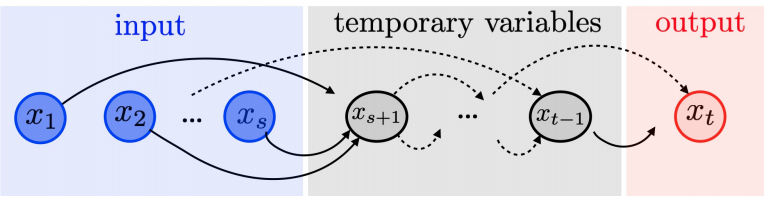
\includegraphics[width=.8\textwidth]{computational_graph.png}
  \\
  \vspace{0.3cm}
  \begin{footnotesize}
    SOURCE:~\citeonline[p.~31]{peyre}.
  \end{footnotesize}
  \label{fig:compgraph}
\end{figure}

The computational graph, \autoref{fig:compgraph}, has the role of
represent the linking of the variables involved in \(f_{k}\) to
\(\mathbf{x}_{k}\). The evaluation of \(f(\mathbf{x})\) corresponds to a
forward traversal of this graph. Now, how we evaluate \(f\) through the
graph? Via one of the AD modes.

\subsection{Forward Mode}

The forward mode correspond to the usual way of computing differentials.
The method initialize with the derivative of the input nodes
\[
  \frac{\partial\mathbf{x}_{1}}{\partial\mathbf{x}_{1}} =
  \text{Id}_{n_{1} \times n_{1}},\quad
  \frac{\partial\mathbf{x}_{2}}{\partial\mathbf{x}_{1}} =
  \mathbf{0}_{n_{2} \times n_{1}},\quad
  \frac{\partial\mathbf{x}_{s}}{\partial\mathbf{x}_{1}} =
  \mathbf{0}_{n_{s} \times n_{1}},
\]
and then iteratively make use of the following recursion formula
\begin{align*}
  &\forall~k = s + 1,~\dots,~t,\\
  &\frac{\partial\mathbf{x}_{k}}{\partial\mathbf{x}_{1}} =
    \sum_{l~\in~\text{father}(k)}
    \frac{\partial\mathbf{x}_{k}}{\partial\mathbf{x}_{l}}\times
    \frac{\partial\mathbf{x}_{l}}{\partial\mathbf{x}_{1}} =
    \sum_{l~\in~\text{father}(k)}
    \frac{\partial}{\partial\mathbf{x}_{l}}
    f_{k}(\mathbf{x}_{1},~\dots,~\mathbf{x}_{k-1})\times
    \frac{\partial\mathbf{x}_{l}}{\partial\mathbf{x}_{1}}.
\end{align*}
The notation ``father(\(k\))'' denotes the nodes \(l < k\) of the graph
that are connected to \(k\). We make use of \citeonline[p.~32]{peyre}'s
simple example.

\noindent\textbf{Example.}\hspace{.5cm}
Consider the function
\[
  f(x, y) = y\log(x) + \sqrt{y\log(x)}
\]
with the corresponding computational graph being displayed in
\autoref{fig:excompgraph}.

\begin{figure}[H]
  \setlength{\abovecaptionskip}{.0001pt}
  \caption{EXAMPLE OF A SIMPLE COMPUTATIONAL GRAPH}
  \vspace{0.3cm} \centering
  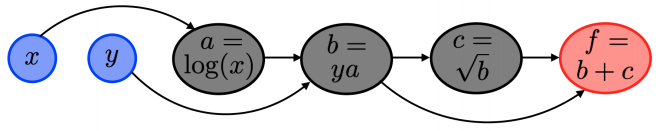
\includegraphics[width=.8\textwidth]{ex-computational_graph.png}
  \\
  \vspace{0.3cm}
  \begin{footnotesize}
    SOURCE:~\citeonline[p.~33]{peyre}.
  \end{footnotesize}
  \label{fig:excompgraph}
\end{figure}

The forward mode iterations to compute the derivative w.r.t. \(x\)
following the computational graph, is given by
\begin{align*}
  \frac{\partial x}{\partial x} &= 1, \quad
  \frac{\partial y}{\partial x} = 0\\
  \frac{\partial a}{\partial x} &=
  \frac{\partial a}{\partial x} \frac{\partial x}{\partial x} =
  \frac{1}{x} \frac{\partial x}{\partial x} \qquad
  &\{x \mapsto a = \log(x)\}\\
  \frac{\partial b}{\partial x} &=
  \frac{\partial b}{\partial a} \frac{\partial a}{\partial x} +
  \frac{\partial b}{\partial y} \frac{\partial y}{\partial x} =
  y \frac{\partial a}{\partial x} + 0 \qquad
  &\{(y, a) \mapsto b = ya\}\\
  \frac{\partial c}{\partial x} &=
  \frac{\partial c}{\partial b} \frac{\partial b}{\partial x} =
  \frac{1}{2\sqrt{b}} \frac{\partial b}{\partial x} \qquad
  &\{b \mapsto c = \sqrt{b}\}\\
  \frac{\partial f}{\partial x} &=
  \frac{\partial f}{\partial b} \frac{\partial b}{\partial x} +
  \frac{\partial f}{\partial c} \frac{\partial c}{\partial x} =
  1 \frac{\partial b}{\partial x} + 1 \frac{\partial c}{\partial x}
  \qquad &\{(b, c) \mapsto f = b + c\}
\end{align*}
To compute the derivative w.r.t. \(y\) we run another forward process
\begin{align*}
  \frac{\partial x}{\partial y} &= 0, \quad
  \frac{\partial y}{\partial y} = 1\\
  \frac{\partial a}{\partial y} &=
  \frac{\partial a}{\partial x} \frac{\partial x}{\partial y} = 0 \qquad
  &\{x \mapsto a = \log(x)\}\\
  \frac{\partial b}{\partial y} &=
  \frac{\partial b}{\partial a} \frac{\partial a}{\partial y} +
  \frac{\partial b}{\partial y} \frac{\partial y}{\partial y} =
  0 + a \frac{\partial y}{\partial y}\qquad
  &\{(y, a) \mapsto b = ya\}\\
  \frac{\partial c}{\partial y} &=
  \frac{\partial c}{\partial b} \frac{\partial b}{\partial y} =
  \frac{1}{2\sqrt{b}} \frac{\partial b}{\partial y} \qquad
  &\{b \mapsto c = \sqrt{b}\}\\
  \frac{\partial f}{\partial y} &=
  \frac{\partial f}{\partial b} \frac{\partial b}{\partial y} +
  \frac{\partial f}{\partial c} \frac{\partial c}{\partial y} =
  1 \frac{\partial b}{\partial y} + 1 \frac{\partial c}{\partial y}
  \qquad &\{(b, c) \mapsto f = b + c\}
\end{align*}

\subsection{Reverse Mode}

Instead of evaluating the differentials for all the input nodes, which
is problematic for a large number of nodes, the reverse mode evaluates
the differentials of the output node w.r.t. all the inner nodes.

The method is based on a backward adjoint chain rule and initialize with
the derivative of the final node
\[
  \frac{\partial\mathbf{x}_{t}}{\partial\mathbf{x}_{t}} =
  \text{Id}_{n_{t} \times n_{t}},
\]
and then, from the last to the first node, iteratively make use of the
following recursion formula
\begin{align*}
  &\forall~k = t - 1,~t - 2,~\dots,~1,\\
  &\frac{\partial\mathbf{x}_{t}}{\partial\mathbf{x}_{k}} =
    \sum_{m~\in~\text{son}(k)}
    \frac{\partial\mathbf{x}_{t}}{\partial\mathbf{x}_{m}}\times
    \frac{\partial\mathbf{x}_{m}}{\partial\mathbf{x}_{k}} =
    \sum_{m~\in~\text{son}(k)}
    \frac{\partial\mathbf{x}_{t}}{\partial\mathbf{x}_{m}}\times
    \frac{\partial}{\partial\mathbf{x}_{k}}
    f_{m}(\mathbf{x}_{1}, \dots, \mathbf{x}_{m}).
\end{align*}
The notation ``son(\(k\))'' denotes the nodes \(m < k\) of the graph
that are connected to \(k\). To be clear, the same simple example.

\noindent\textbf{Example.}\hspace{.5cm}
Consider, again, the function
\[
  f(x, y) = y\log(x) + \sqrt{y\log(x)}.
\]
The iterations of the reverse mode is given by
\begin{align*}
  \frac{\partial f}{\partial f} &= 1\\
  \frac{\partial f}{\partial c} &=
  \frac{\partial f}{\partial f} \frac{\partial f}{\partial c} =
  \frac{\partial f}{\partial f} 1\qquad &\{c \mapsto f = b + c\}\\
  \frac{\partial f}{\partial b} &=
  \frac{\partial f}{\partial c} \frac{\partial c}{\partial b} +
  \frac{\partial f}{\partial f} \frac{\partial f}{\partial b} =
  \frac{\partial f}{\partial c} \frac{1}{2\sqrt{b}} +
  \frac{\partial f}{\partial f} 1\qquad
  &\{b \mapsto c = \sqrt{b},~b \mapsto f = b + c\}\\
  \frac{\partial f}{\partial a} &=
  \frac{\partial f}{\partial b} \frac{\partial b}{\partial a} =
  \frac{\partial f}{\partial b} y\qquad &\{a \mapsto b = ya\}\\
  \frac{\partial f}{\partial y} &=
  \frac{\partial f}{\partial b} \frac{\partial b}{\partial y} =
  \frac{\partial f}{\partial b} a \qquad &\{y \mapsto b = ya\}
\end{align*}
\begin{align*}
  \frac{\partial f}{\partial x} &=
  \frac{\partial f}{\partial a} \frac{\partial a}{\partial x} =
  \frac{\partial f}{\partial a} \frac{1}{x} \hspace{6.5cm}
  &\{x \mapsto a = \log(x)\}
\end{align*}
This is the advantage of reverse mode over the forward mode. A single
traversal over the computational graph allows to compute both
derivatives w.r.t. \(x\) and \(y\), while the forward mode necessities
two processes.

An drawback of the reverse mode is the need to store the entire
computational graph, which is needed for the reverse sweep. In
principle, storage of this graph is not too difficult to implement.
However, the main benefit of AD is higher accuracy, and in many
applications the cost is not critical.

\section{TMB: TEMPLATE MODEL BUILDER}
\label{cap:tmb}

Note that the goal of AD is not to define an efficient computational
graph, it is up to the user to provide it. However, computing an
efficient graph associated to a mathematical formula is a complicated
combinatorial problem. Thus, since our goal is to be able to fit our
desired statistical models, a computational tool able to efficiently
define and implement this computational graph is make necessary. To
solve this and many other tasks, we have the Template Model Builder
(TMB) developed by \citeonline{TMB}.

TMB \url{ http://tmb-project.org} is an \texttt{R} \cite{R18} package
for fitting statistical latent variable models to data, inpired by AD
Model Builder (ADMB) and developed by \citeonline{ADMB}. ADMB is a
statistical application for fitting nonlinear statistical models and
solve optimization problems, that implements AD using \texttt{C++}
classes and a native template language. Unlike most \texttt{R} packages,
in TMB the model is formulated in \texttt{C++}. This characteristic
provides great flexibility but requires some familiarity with the
\texttt{C}/\texttt{C++} programming language. With TMB a user should be
able to quickly implement complex latent effect models through simple
\texttt{C++} templates.

In this chapter we describe step-by-step all the processes involved in
the creation and parameter estimation of a GLMM. With TMB all this is
put in practice in an efficient and robust fashion.

The user needs to provide just the joint likelihood function writing in
a \texttt{C++} template. When the model presents latent effects, during
the compilation the latent effects will be integrated out via an
efficient Laplace approximation routine with a Newton algorithm inside,
and the marginal log-likelihood gradient will be also computed and
returned. The marginal log-likelihood will be returned into an
\texttt{R} object that can then be optimized using the user's favorite
quasi-Newton routine, available in \texttt{R}. To accomplish all that,
TMB combines some state-of-art software

\begin{itemize}
\item \texttt{CppAD}, a \texttt{C++} AD package
  \url{https://coin-or.github.io/CppAD/};
\item \texttt{Eigen} \cite{eigen}, a \texttt{C++} templated
  matrix-vector library;
\item \texttt{CHOLMOD}, sparse matrix routines available from
  \texttt{R}, used to obtain an efficient implementation of the Laplace
  approximation with exact derivatives
  \url{https://developer.nvidia.com/cholmod};
\item Parallelism through \texttt{BLAS}: Basic Linear Algebra
  Subprograms \url{http://www.netlib.org/blas/}.
\end{itemize}

Also, some of its key characteristics are

\begin{itemize}
\item TMB employs AD to calculate first and second order derivatives of
  the likelihood function or any objective function in \texttt{C++};
\item The objective function, and its derivatives, can be called from
  \texttt{R}. Hence, parameter estimation via \texttt{optim()} or
  \texttt{nlminb()} is easy to be performed;
\item Standard deviations of any parameter, or derived parameter, can be
  obtained via the \textit{delta method}.
\end{itemize}

Here we focus on GLMMs, but basically any statistical model with a
latent structure (or not), linear (or not), can be fitted with TMB. In
times of \textit{big data}, and with the TMB's authors having a
professional preference for state-of-space and spatial models, TMB has
also automatic sparseness detection.and some other nice built tools. Pre
and post-processing of data should be done in \texttt{R}.

A TMB Users' mailing list exists, and it is extremely helpful for taking
doubts and questions \url{https://groups.google.com/g/tmb-users}. Also,
a very didactic and comprehensive documentation with several examples is
available online
\url{https://kaskr.github.io/adcomp/_book/Tutorial.html}.

% END ==================================================================